\documentclass[10pt,a4paper]{amsart}
\usepackage[utf8]{inputenc}
\usepackage[english]{babel}
\usepackage[mathcal]{euscript}
\usepackage{mathrsfs}  
\usepackage{amsmath}
\usepackage{amsfonts}
\usepackage{mathrsfs}  
\usepackage{amssymb}
\usepackage{stmaryrd}
\usepackage{graphicx}
\usepackage{mathtools}
\usepackage{pgfplots}
\usepackage{xfrac}
\usepackage{listings}
\usepackage{xcolor}
\usepackage{lstlinebgrd}
\usepackage{ebproof}
\usepackage{graphicx,float}
\usepackage[colorlinks=true, linkcolor=cyan, urlcolor=cyan, citecolor=cyan]{hyperref}
\usepackage[shortlabels]{enumitem}
\usepackage[textsize=tiny,textwidth=45]{todonotes}

\newcommand{\klcomp}{\star}
\newcommand{\parI}{\mathop{\bowtie}}
\newcommand{\seqI}{\mathop{\triangleright}}
\DeclareMathOperator{\demon}{\square}
\DeclareMathOperator{\angel}{\Diamond}
\makeatletter
\DeclareRobustCommand{\iscircle}{\mathord{\mathpalette\is@circle\relax}}
\newcommand\is@circle[2]{%
  \begingroup
  \sbox\z@{\raisebox{\depth}{$\m@th#1\bigcirc$}}%
  \sbox\tw@{$#1\square$}%
  \resizebox{!}{\ht\tw@}{\usebox{\z@}}%
  \endgroup
}
\makeatother
\DeclareMathOperator{\statt}{\iscircle_\prog{p}}
\newcommand{\schfont}[1]{\mathcal{#1}}
\newcommand{\sch}{\schfont{S}}
\newcommand{\conv}[1]{\mathrm{conv}\, {#1}}
%%%%%%%%%%%%% Macros
\newcommand{\renato}[1]{\textcolor{teal}{RN Note: #1}}
\newcommand{\codiag}{\triangledown}
%%%% Categories
\newcommand{\catfont}[1]{\mathsf{#1}}
\newcommand{\cop}{\catfont{op}}
\newcommand{\Law}{\catfont{Law}}
\newcommand{\catV}{\catfont{V}}
\newcommand{\catX}{\catfont{X}}
\newcommand{\catC}{\catfont{C}}
\newcommand{\catCat}{\catfont{C}}
\newcommand{\catCop}{\catfont{C^{op}}}
\newcommand{\catD}{\catfont{D}}
\newcommand{\catE}{\catfont{E}}
\newcommand{\catA}{\catfont{A}}
\newcommand{\catB}{\catfont{B}}
\newcommand{\catP}{\catfont{P}}
\newcommand{\catMet}{\catfont{Met}}
\newcommand{\catCPTP}{\catfont{CPTP}}
\newcommand{\catCPS}{\catfont{CPS}}
\newcommand{\catCP}{\catfont{CP}}
\newcommand{\catQ}{\catfont{Q}}
\newcommand{\catSet}{\catfont{Set}}
\newcommand{\catFinSet}{\catfont{FinSet}}
\newcommand{\catPO}{\catfont{PO}}
\newcommand{\catCompFunc}{\catfont{CompFunc}}
\newcommand{\catBan}{\catfont{Ban}}
\newcommand{\catVect}{\catfont{CVect}}
\newcommand{\WstarCPSU}{\catfont{Wstar_{CPSU}}}
\newcommand{\WstarCPSUop}{\left(\catfont{Wstar_{CPSU}}\right)^{\catfont{op}}}
\newcommand{\catI}{\catfont{I}}
\newcommand{\Set}{\catfont{Set}}
\newcommand{\Top}{\catfont{Top}}
\newcommand{\Pos}{\catfont{Pos}}
\newcommand{\Inj}{\catfont{Inj}}
\newcommand{\Det}{\catfont{RMhat}}
\newcommand{\CoAlg}[1]{\catfont{CoAlg}\left (#1 \right )}
\newcommand{\Mon}{\catfont{Mon}}
\newcommand{\Mnd}{\catfont{Mnd}(\catC)}
\newcommand{\SMnd}{\catfont{Mnd}(\Set)}
\newcommand{\CLat}{\catfont{CLat}}
\newcommand{\SLat}{\catfont{SLat}}
\newcommand{\Stone}{\catfont{Stone}}
\newcommand{\Spectral}{\catfont{Spectral}}
\newcommand{\CompHaus}{\catfont{CompHaus}}
\newcommand{\Subs}[2]{\catfont{Sub}_{}}
\newcommand{\Cone}{\catfont{Cone}}
\newcommand{\LCone}{\catfont{LCone}}
\newcommand{\StComp}{\catfont{StablyComp}}
\newcommand{\PosC}{\catfont{PosComp}}
\newcommand{\Haus}{\catfont{Haus}}
\newcommand{\Meas}{\catfont{Meas}}
\newcommand{\Coh}{\catfont{CohDom}}
\newcommand{\Ord}{\catfont{Ord}}
\newcommand{\Dcpo}{\catfont{DCPO}}
\newcommand{\Dom}{\catfont{Dom}}
\newcommand{\EndoC}{[\catC,\catC]}
\newcommand{\Dcpop}{\catfont{DCPO}^\catfont{p}}
%% General functors
\newcommand{\funfont}[1]{#1}
\newcommand{\funF}{\funfont{F}}
\newcommand{\funU}{\funfont{U}}
\newcommand{\funG}{\funfont{G}}
\newcommand{\funT}{\funfont{T}}
\newcommand{\funI}{\funfont{I}}
%% Particular kinds of functors
\newcommand{\sfunfont}[1]{\mathrm{#1}}
\newcommand{\Pow}{\sfunfont{P}}
\newcommand{\PP}{\sfunfont{V}}
\newcommand{\Dist}{\sfunfont{V}_{=1,\omega}}
\newcommand{\PDist}{\sfunfont{V}_{\leq 1,\omega}}
\newcommand{\Maybe}{\sfunfont{M}}
\newcommand{\List}{\sfunfont{L}}
\newcommand{\UForg}{\sfunfont{U}}
\newcommand{\Forg}[1]{\sfunfont{U}_{#1}}
\newcommand{\Id}{\sfunfont{Id}}
\newcommand{\Vie}{\sfunfont{V}}
\newcommand{\Disc}{\funfont{D}}
\newcommand{\Weight}{\sfunfont{W}}
\newcommand{\homf}{\sfunfont{hom}}
\newcommand{\Yoneda}{\sfunfont{Y}}
%% Diagram functors
\newcommand{\Diag}{\mathscr{D}}
\newcommand{\KDiag}{\mathscr{K}}
\newcommand{\LDiag}{\mathscr{L}}
%% Monads
\newcommand{\monadfont}[1]{\mathbb{#1}}
\newcommand{\monadT}{\monadfont{T}}
\newcommand{\monadS}{\monadfont{S}}
\newcommand{\monadU}{\monadfont{U}}
\newcommand{\monadH}{\monadfont{H}}
\newcommand{\str}{\mathrm{str}}
%% Adjunctions
\newcommand\adjunct[2]{\xymatrix@=8ex{\ar@{}[r]|{\top}\ar@<1mm>@/^2mm/[r]^{{#2}}
& \ar@<1mm>@/^2mm/[l]^{{#1}}}}
\newcommand\adjunctop[2]{\xymatrix@=8ex{\ar@{}[r]|{\bot}\ar@<1mm>@/^2mm/[r]^{{#2}}
& \ar@<1mm>@/^2mm/[l]^{{#1}}}}
%% Retractions
\newcommand\retract[2]{\xymatrix@=8ex{\ar@{}[r]|{}\ar@<1mm>@/^2mm/@{^{(}->}[r]^{{#2}}
& \ar@<1mm>@/^2mm/@{->>}[l]^{{#1}}}}
%% Limits
\newcommand{\pv}[2]{\langle #1, #2 \rangle}
\newcommand{\limt}{\mathrm{lim}}
\newcommand{\pullbackcorner}[1][dr]{\save*!/#1+1.2pc/#1:(1,-1)@^{|-}\restore}
\newcommand{\pushoutcorner}[1][dr]{\save*!/#1-1.2pc/#1:(-1,1)@^{|-}\restore}
%% Colimits
\newcommand{\colim}{\mathrm{colim}}
\newcommand{\inl}{\mathrm{inl}}
\newcommand{\inr}{\mathrm{inr}}
%% Distributive categories
\newcommand{\distr}{\mathrm{dist}}
\newcommand{\undistr}{\mathrm{undist}}
%% Closedness
\newcommand{\curry}[1]{\mathrm{curry}{#1}}
\newcommand{\app}{\mathrm{app}}
%% Misc. operations
\newcommand{\const}[1]{\underline{#1}}
\newcommand{\comp}{\cdot}
\newcommand{\id}{\mathrm{id}}
\newcommand{\sw}{\mathrm{sw}}
\newcommand{\spt}{\mathrm{sp}}
\newcommand{\sh}{\mathrm{sh}}
\newcommand{\jn}{\mathrm{jn}}
\newcommand{\dist}{\mathrm{dist}}
\newcommand{\unfold}{\mathrm{unfold}}
\newcommand{\fold}{\mathrm{fold}}
%% Factorisations
\newcommand{\EClass}{E}
\newcommand{\MClass}{M}
\newcommand{\MConeClass}{\mathcal{M}}
%%%%%%%%%%%%%%%% End of Categorical Stuff

%%%% Misc
%% Operations
\newcommand{\blank}{\, - \,}
\newcommand{\sem}[1]{\left \llbracket #1 \right \rrbracket}
\newcommand{\asem}[1]{ \llparenthesis #1 \rrparenthesis}
\newcommand{\closure}[1]{\overline{#1}}
\DeclareMathOperator{\img}{\mathrm{im}}
\DeclareMathOperator{\dom}{\mathrm{dom}}
\DeclareMathOperator{\codom}{\mathrm{codom}}
%% Sets of numbers
\newcommand{\Nats}{\mathbb{N}}
\newcommand{\Reals}{\mathbb{R}}
\newcommand{\Rats}{\mathbb{Q}}
\newcommand{\Rz}{\Reals_{\geq 0}}
\newcommand{\Complex}{\mathbb{C}}
%% Writing
\newcommand{\cf}{\emph{cf.}}
\newcommand{\ie}{\emph{i.e.}}
\newcommand{\eg}{\emph{e.g.}}
\newcommand{\df}[1]{\emph{\textbf{#1}}}
%%%%%%%%%%%%%%%% End of Misc

%%%% Programming Stuff
%% Types
\newcommand{\typefont}[1]{\mathbb{#1}}
\newcommand{\typeOne}{1}
\newcommand{\typeTwo}{2}
\newcommand{\typeA}{\typefont{A}}
\newcommand{\typeB}{\typefont{B}}
\newcommand{\typeC}{\typefont{C}}
\newcommand{\typeV}{\typefont{V}}
\newcommand{\typeD}{\typefont{D}}
\newcommand{\typeE}{\typefont{E}}
\newcommand{\typeF}{\typefont{F}}
\newcommand{\typeI}{\typefont{I}}
%% RuleName
\newcommand{\rulename}[1]{(\mathrm{#1})}
%% Sequents
\newcommand{\jud}{\vdash}
\newcommand{\vljud}{\triangleright}
\newcommand{\cojud}{\vdash_{\co}}
\newcommand{\vl}{\mathtt{v}}
\newcommand{\co}{\mathtt{c}}
% Program font
\newcommand{\prog}[1]{\ensuremath{\tt #1}}
\newcommand{\blue}[1]{\textcolor{blue}{#1}}
\newcommand{\pseq}[3]{#1 \leftarrow #2; #3}
\newcommand{\ppm}[4]{(#1,#2) \leftarrow #3; #4}
\newcommand{\pinl}[1]{\prog{inl}(#1)}
\newcommand{\pinr}[1]{\prog{inr}(#1)}
\newcommand{\pcase}[5]{\prog{ case } #1 \prog{ \hspace{2pt} of \hspace{2pt} } \pinl{#2} \Rightarrow #3 ; \pinr{#4} \Rightarrow #5}
%% Sets of terms
\newcommand{\ValuesBP}[2]{\mathsf{Values}(#1, #2)}
\newcommand{\TermsBP}[2]{\mathsf{Terms}(#1, #2)}
\newcommand{\closValP}[1]{\ValuesBP{\emptyset}{#1}}
\newcommand{\closTermP}[1]{\TermsBP{\emptyset}{#1}}
\newcommand{\closVal}{\closValP{\typeA}}
\newcommand{\closTerm}{\closTermP{\typeA}}
%% Contextual equivalence
\newcommand{\ctxeq}{\equiv_{\prog{ctx}}}

%%%% End of Programming Stuff
\newcommand{\Shuff}{\mathrm{Sf}}

%%%% Domain theory
\newcommand{\upclos}{\mathord{\uparrow}}
\newcommand{\dwclos}{\mathord{\downarrow}}

%%%% Quantum stuff
\newcommand{\Hilb}{\catfont{Hilb}}
\newcommand{\tr}{\text{Tr}}

%%%% Norms
\newcommand{\euclideannorm}[1]{\left\lVert #1  \right\rVert_{2}}
\newcommand{\spectralnorm}[1]{\left\lVert #1  \right\rVert_{\infty}}
\newcommand{\tracenorm}[1]{\left\lVert #1  \right\rVert_{1}}
\newcommand{\diamondnorm}[1]{\left\lVert #1  \right\rVert_{\diamondsuit}}
\newcommand{\lonenorm}[1]{\left\lVert #1  \right\rVert_{ L^{1} }}
\newcommand{\gentracenorm}[1]{\left\lVert #1  \right\rVert_{ L^\infty }}
\newcommand{\gendiamondnorm}[1]{\left\lVert #1  \right\rVert_{ \diamondsuit \text{ gen}}}
\newcommand{\opnorm}[1]{\left\lVert #1  \right\rVert_{\text{op}}}
\newcommand{\norm}[1]{\left\lVert #1  \right\rVert}
\newcommand{\cbnorm}[1]{\left\lVert #1  \right\rVert_{\text{cb}}}
\newcommand{\projnorm}[1]{\left\lVert #1  \right\rVert_{\pi}}

%%%% Tensor
\newcommand{\projtensor}{\widehat{\otimes}_\pi}

\usepackage[left=2cm,right=2cm,top=2cm,bottom=2cm]{geometry}
\usepackage{tcolorbox}
\usepackage{braket}
\usepackage{quantikz}
\usepackage{tikz-cd}
\linespread{1.10}
\author{\dots}
\title{Notes}

\lstset{
language=C,
showstringspaces=false,
keywordstyle=\color{blue},
basicstyle=\fontsize{10}{13}\ttfamily,
emph={exit,blue,unif,then,wait},emphstyle=\color{blue},
breaklines=true,
escapeinside={*@}{*@}
}


\usepackage{proof}
\usepackage{amsthm}
\usepackage[all]{xy}
%for definition
\theoremstyle{definition}
\newtheorem{definition}{Definition}[section]

%for examples
\theoremstyle{definition}
\newtheorem{example}[definition]{Example}

%lemmas
\theoremstyle{definition}
\newtheorem{lemma}[definition]{Lemma}

%proposition
\theoremstyle{definition}
\newtheorem{proposition}[definition]{Proposition}
%corollary
\theoremstyle{definition}
\newtheorem{corollary}[definition]{Corollary}

%theorem
\theoremstyle{definition}
\newtheorem{theorem}[definition]{Theorem}

% Renato's macros
\newcommand{\until}{\> \textcolor{blue}{\prog{for}} \>}
\newcommand{\then}{\textcolor{blue}{then}}
\newcommand{\progife}[3]{{ \blue{\prog{if}} \> #1 \> \blue{\prog{then}} \> 
{\prog #2} \> \blue{\prog{else}} \> {\prog #3}}}
\newcommand{\progwhile}[2]{{\blue{\prog{while}} \>  #1 \> \blue{\prog{do}} \> \{ \> {#2}  \> \}}}
\newcommand{\scomp}{\, \blue{;} \,}
\newcommand{\prem}[1]{(\text{if\/ }#1)}
\newcommand{\nline}{\vspace{-5mm}}
\newcommand{\ssto}[1][]{~\to^{#1}~}
\newcommand{\bsto}{~\Downarrow~}
\newcommand{\stp}{\mathit{stop}}
\newcommand{\skp}{\mathit{skip}}
\newcommand{\err}{\mathit{err}}
\providecommand{\comma}{,\operatorname{}\linebreak[1]}		% possibly line-beaking comma
\newcommand{\sep}{\kern1pt\comma\kern-1pt}
\newcommand{\lrule}[3]{\textbf{#1}\quad\frac{#2}{#3}}
\newcommand{\ptt}{{\prog tt}}
\newcommand{\pff}{{\prog ff}}
\newcommand{\unif}{{\prog \blue{unif}}}
\newcommand{\meas}[1]{\mathcal{M}(#1)}
\newcommand{\pmap}{ \xrightharpoonup{\hspace{0.1cm}} }

\begin{document}
\title{Quantum stuff}
\maketitle
%\tableofcontents
\section{Lambda-calculus with conditionals}

\subsection{Syntax}

Considering a class $G$ of ground types, the grammar of types for linear lambda calculus with conditionals corresponds to:

\begin{equation*} \label{eq:grammartypes}
  \centering
   \mathbb{A} ::= X \in G \hspace{3 pt} \vert \hspace{3 pt} \mathbb{I}  \hspace{3 pt}  \vert \hspace{3 pt} \mathbb{A}  \otimes  \mathbb{A} \hspace{3 pt} \vert  \hspace{3 pt} \mathbb{A}  \oplus \mathbb{A} \hspace{3 pt}  \vert  \hspace{3 pt} \mathbb{A} \multimap  \mathbb{A}
  \end{equation*}

The term formation rules for conditionals are depicted in \autoref{fig:typing_rules_cond}. 

\begin{figure}[H]
    \begin{equation*}
    \begin{aligned}
    &\hspace{10pt}
    %
    \begin{prooftree}
        \hypo{\Gamma \vljud v: \typeA}
        \infer1[(inl)]{\Gamma \vljud \inl_{\typeB}(v): \typeA \oplus \typeB}
    \end{prooftree}
    %
    \hspace{30pt}
    %
    \begin{prooftree}
        \hypo{\Gamma \vljud v: \typeB}
        \infer1[(inr)]{\Gamma \vljud \inr_{\typeA}(v): \typeA \oplus \typeB}
    \end{prooftree} 
    %
    \\[20pt]
    &\hspace{-20pt}
    %
    \begin{prooftree}
        \hypo{\Gamma \vljud v: \typeA \oplus \typeB}
        \hypo{\Delta, x: \typeA \vljud w: \typeD}
        \hypo{\Delta, y: \typeB \vljud u: \typeD}
        \hypo{E \in \Shuff(\Gamma; \Delta)}
        \infer4[(case)]{E \vljud \text{case } v\,
        \{\inl_{\typeB}(x) 
            \Rightarrow w ; \,
          \inr_{\typeA}(y) \Rightarrow u
        \}: \typeD}
    \end{prooftree}
    %
    \\[10pt]
    \end{aligned}
    \end{equation*}
    \caption{Term formation rules for conditionals}
    \label{fig:typing_rules_cond}
\end{figure}
The rules presented in Figure \ref{fig:typing_rules_cond} enjoy the following
properties.

\begin{theorem} \label {theorem:unique_der}
   Lambda calculus with conditionals has the following properties:
   \begin{enumerate}
     \item\label{perm} for all judgements $\Gamma \vljud v$ and $\Gamma'
             \vljud v$, te($\Gamma$) $\simeq_{\pi}$  te($\Gamma'$); 
     %
     \item\label{type} additionally if $\Gamma \vljud v: \typeA,
       \Gamma' \vljud v: \typeA'$, and $\Gamma \simeq_{\pi}
       \Gamma'$, then $\typeA$ must be equal to $\typeA'$;
     %
     \item\label{der} all judgements $\Gamma \vljud v:\typeA$ have a unique derivation.
\end{enumerate}
\end{theorem}
%
\begin{proof}
It follows in all three cases from induction over the length of derivation
trees. 

Let us focus first on Property~\eqref{perm}. The case of the rules concerning
injections is direct. As for rule~$\rulename{cond}$ take two contexts $E$ and
$E'$ for the same conditional. According to this rule we obtain contexts
$\Gamma$, $\Gamma'$, $\Delta$, $\Delta'$ such that $E \in
\Shuff(\Gamma;\Delta)$ and $E' \in \Shuff(\Gamma';\Delta')$. It follows from
induction that  $\Gamma \simeq_\pi \Gamma'$ and $\Delta \simeq_\pi \Delta'$,
and the proof is then obtained from the sequence of equivalences,
\begin{align*}
        \text{te}(E) & \simeq_\pi \text{te}(\Gamma, \Delta) 
        \\
        & \simeq_\pi \text{te}(\Gamma', \Delta')
        \\
        & \simeq_\pi \text{te}(E')
\end{align*}
Concerning Property~\eqref{type}, the case of the rules concerning injections
is direct and the case of rule~$\rulename{cond}$ is a corollary of
Property~\eqref{perm}. Finally let us consider Property~\eqref{der}. Again the
case concerning injections is direct and we thus focus only on
rule~$\rulename{cond}$. According to this rule we obtain contexts $\Gamma$,
$\Gamma'$, $\Delta$, $\Delta'$ such that $E \in \Shuff(\Gamma;\Delta)$ and $E
\in \Shuff(\Gamma';\Delta')$. By an appeal to Property~\eqref{perm} we also
obtain $\Gamma \simeq_\pi \Gamma'$ and $\Delta \simeq_\pi \Delta'$, and thus
since shuffling preserves relative orders we obtain $\Gamma = \Gamma'$ and
$\Delta = \Delta'$. The proof then follows by induction.
\end{proof}

\begin{lemma}[Exchange and Subsitution]
\label{lem:exh_and_sub} 
For every judgement $\Gamma,x: \typeA, y: \typeB, \Delta \vljud v: \typeD$ the
judgement $\Gamma, y:\mathbb{B}, x:\mathbb{A}, \Delta \vljud v:
\typeD$ is derivable. Not only this, given judgements  $\Gamma,x:\typeA \vljud
v: \typeB$ and $\Delta \vljud w: \typeA$ the judgement $\Gamma, \Delta \vljud
v[w/x]: \typeB$ is also derivable.
\end{lemma}


\begin{proof}
We start with the exchange property which follows by induction over the length
of derivation trees. The rules that involve injections are direct.  The rule
$\rulename{case}$ calls for case distinction, more specifically we  distinguish
between the cases in which both variables ($x : \typeA$ and $y : \typeB$) are
in $\Gamma$, both are in $\Delta$, and otherwise. The first two cases follow
straightforwardly by induction and the definition of a shuffle. For the third
case consider a judgement $E_1,x : \typeA, y : \typeB, E_2 \vljud \text{case }
v\, \{\inl_{\typeF}(a) \Rightarrow w ; \, \inr_{\typeE}(b) \Rightarrow u \}:
\typeD$, and assume with no loss of generality that $\Gamma$ is of the form
$\Gamma_1, x : \typeA, \Gamma_2$ and $\Delta$ of the form $\Delta_1, y :
\typeB, \Delta_2$. The proof now follows directly from the implication,
\[
        E_1, x : \typeA, y : \typeB, E_2 \in \Shuff(\Gamma_1, x : \typeA, \Gamma_2 ; \,
        \Delta_1, y : \typeB, \Delta_2)
        \Longrightarrow
        E_1, y : \typeB, x : \typeA, E_2 \in \Shuff(\Gamma_1, x : \typeA, \Gamma_2 ; \,
        \Delta_1, y : \typeB, \Delta_2)
\]
(which holds by the definition of a shuffle).

Finally we now focus on the substitution rule which also follows by induction over the
length of derivation trees. Again the cases involving the injections are direct,
and we thus only detail the proof of rule $\rulename{case}$. Consider then
judgements $E,x : \typeA \vljud \text{case } v\, \{\inl_{\typeD}(a) \Rightarrow
w ; \, \inr_{\typeE}(b) \Rightarrow u \}: \typeB$ and
$Z \vljud t : \typeA$ with $E \in \Shuff(\Gamma; \Delta)$. According to the definition
of a shuffle either $\Gamma$ is of the form $\Gamma_1, x: \typeA$ or $\Delta$ is
of the form $\Delta_1, x : \typeA$. The first case follows directly and the second case
is a corollary of the exchange rule.
\end{proof}

The equational system for the conditionals is shown in Figure
\ref{fig:equations-in-context-cond}.


  \begin{figure}[h!]
    \centering
    \begin{tcolorbox}[colframe=black, colback=white, boxrule=0.6pt, arc=1pt,boxsep=1pt,top=1pt,bottom=1pt, width=0.85 \textwidth]
    \begin{equation*}
        \begin{split}
          &(\beta_{case}^{inl}) \hspace{3pt} \text{ case } 
          \inl_{\typeB}(v) \hspace{2pt} \{ \inl_{\typeB} (x) \Rightarrow w 
          ; \hspace{1pt} \inr_{\typeA} (y) 
          \Rightarrow u\}= w[v/x]
          %
          \\
          %
          &(\beta_{case}^{inr}) \hspace{3pt} \text{ case } 
          \inr_{\typeA}(v) \hspace{2pt} \{ \inl_{\typeB} (x) \Rightarrow w 
          ; \hspace{1pt} \inr_{\typeA} (y) 
          \Rightarrow u\}= u[v/y]
          %
          \\
          %
          %
          & (\eta_{case}) \hspace{3pt} \text{ case } v\ \hspace{2pt} \{\text{inl}_{\mathbb{B}} (y) \Rightarrow w [ \text{inl}_{\mathbb{B}}(y)/x] ; \hspace{1pt} \text{inr}_{\mathbb{A}} (z) \Rightarrow w [ \text{inr}_{\mathbb{A}}(z)/x]\} = w[v/x] 
        \end{split}
    \end{equation*}
    \end{tcolorbox}
    \caption{Equational system for the conditionals}
    \label{fig:equations-in-context-cond}
    \end{figure}


\subsubsection{Linear $\lambda$-calculus and quantum computation}

We now illustrate the use of the previous language for describing quantum
programs. To this effect, we first consider a type \emph{qbit} of qubits, the
basic unit of information in quantum computation. We then regard $\typeI \oplus
\typeI$ to be the type of bits, a common approach not only in quantum
computation~\cite{selinger04} but also in the categorical interpretation of a
`truth-values' object~\cite{johnstone02,cho15}. Next we propound the following
basic quantum operations:  the conversion of a bit into a qubit, $q : \typeI
\oplus \typeI  \to \emph{qbit}$, the measurement of a qubit,
$\emph{meas}:\emph{qbit} \to \typeI \oplus \typeI$, and a pre-determined set of
operations on $n$-qubits, $\emph{U}:\emph{qbit},\ldots,\emph{qbit} \to
\emph{qbit}^{\otimes n}$. The latter set can include for example the Hadamard
gate $H : \emph{qbit} \to \emph{qbit}$, the not-gate $X : \emph{qbit} \to
\emph{qbit}$, or the cnot-gate $CNOT : \emph{qbit},\emph{qbit} \to
\emph{qbit}^{\otimes 2}$. We consider as well a pre-determined set of quantum
states $\ket{\psi} : \typeI \to \emph{qbit}$.  Finally note that the values
\emph{true} and \emph{false} (in the type $\typeI \oplus \typeI$) are regarded to be 
the terms $\inl(\ast)$ and $\inr(\ast)$ respectively.

Let us now apply this machinery to two well-known problems in quantum computation
and quantum information.

\begin{example}[Coin toss]
~\todo[inline]{Descrever aqui como obter valores $p_0$ e $p_1$ para depois
poderem ser usados no próximo exemplo.}
\end{example}

\begin{example}[Quantum state discrimination]

Quantum state discrimination is a pivotal challenge in quantum information,
fundamental to the extraction of classical information from quantum systems.
While orthogonal states can be perfectly distinguished, the same does not apply
to nonorthogonal states. In fact even when the set of possible nonorthogonal
states is known, determining the optimal discrimination strategy is considered
a nontrivial problem.

When distinguishing between two nonorthogonal quantum states, the Helstrom
measurement represents the optimal strategy
\cite{helstromQuantumDetectionEstimation1976}. In the case where both states
are pure, the Helstrom measurement corresponds to a projective measurement
\cite{barnett2009quantum}.  When operating within the computational basis, a
projective measurement can be understood as the application of a unitary
operator followed by a subsequent measurement in the computational basis. Thus
the Helstrom measurement can be interpreted as a unitary transformation applied
to the quantum state, followed by a measurement in the computational basis. 

We will now show how to describe this discrimination task in
$\lambda$-calculus.  Consider two pure states $\ket{\psi_0}$ and
$\ket{\psi_1}$, prepared \emph{a priori} with probabilities $p_0$ and $p_1$,
respectively. Consider as well an operation $U : \emph{qbit} \to \emph{qbit}$ which
corresponds to the basis-change associated with the Helstrom measurement.
The relevant $\lambda$-terms are then:
\begin{align*}
  &\textbf{StatePreparation} =  b: \typeI \oplus \typeI  \vljud  \text{case } b\,
  \{\inl_{\typeB}(x) \Rightarrow \ket{\psi_0} ; \inr_{\typeA}(y) \Rightarrow \ket{\psi_1}\}: \textit{qbit} \\
  &\textbf{HMeasure} =  x : \emph{qbit} \vljud \emph{meas} (\emph{U}(x)): \typeI \oplus \typeI \\
  &\textbf{Discrimination} = (p_0,p_1): \mathbb{I} \oplus \mathbb{I}  \triangleright \textbf{HMeasure} [ \textbf{StatePreparation} [(p_0,p_1)/ b] / x] : \mathbb{I} \oplus \mathbb{I}
\end{align*}
\end{example}


\begin{example}[Quantum teleportation]
\cite{bennett1993teleporting} introduced the concept of quantum teleportation,
a protocol that allows the transfer of  unknown quantum states between distant
parties.  The quantum teleportation protocol is a fundamental building block of
quantum communication, quantum computation, and quantum networks, its
applications ranging from secure quantum communication to distributed quantum
computing
\cite{briegel1998quantum,gottesman1999demonstrating,kimble2008quantum}.
Conceptually it can be described as follows: Alice and Bob share an entangled
pair of qubits, specifically in a Bell state. Alice keeps the first qubit and
Bob the second. Moreover, Alice has a qubit in an unknown state $\ket{\psi}$
that she wants to send to Bob.  Alice entangles her qubit and the first qubit
in the Bell state, and then measures both. The result of this measurement is
two classical bits that Alice then sends to Bob though a classical channel.
Based on the measurement results, Bob applies a correction to his qubit so it
matches the initial state $\ket{\psi}$.  The circuit corresponding to the
implementation of quantum teleportation is depicted in \autoref{fig:teleport}.


\begin{figure} [H]
  \centering
  \begin{quantikz} [column sep=0.2cm, row sep=0.5cm] 
      \lstick{$\ket{\psi}$}  & \qw &\qw & \qw & \qw & \qw& \ctrl{1}\gategroup[2,steps=4,style={dashed,rounded
      corners,fill=blue!20, inner
      xsep=2pt},background,label style={label
      position=below,anchor=north,yshift=-0.2cm}]{{\sc
      BellMeasure}} & \gate{H} & \qw & \meter{} & \setwiretype{c}  &  & \gategroup[3,steps=4,style={dashed,rounded
      corners,fill=blue!20, inner
      xsep=2pt},background,label style={label
      position=below,anchor=north,yshift=-0.2cm}]{{\sc
      Correction}}  &  & & \ctrl[vertical
wire=c]{2}  \\
      \lstick {$\ket{0}$}  &\gate{H}\gategroup[2,steps=3,style={dashed,rounded
      corners,fill=blue!20, inner
      xsep=2pt},background,label style={label
      position=below,anchor=north,yshift=-0.2cm}]{{\sc
      EPR}} & \qw  & \ctrl{1}& \qw & \qw & \targ{} & \qw & \qw & \meter{} & \setwiretype{c} & & & \ctrl[vertical
wire=c]{1} \\
      \lstick{$\ket{0}$}  &  \qw & \qw &  \targ{} & \qw &\qw&\qw & \qw & \qw& \qw & \qw & \qw &  \qw & \gate{X} & \qw & \gate{Z} 
 \end{quantikz}
  \caption{Quantum Teleportation Protocol}
  \label{fig:teleport}
\end{figure}
We first describe each of the rectangles filled in blue separately, and using
standard quantum gate operations, namely $H: \emph{qbit} \to \emph{qbit}$, $X:
\emph{qbit} \to  \emph{qbit}$, $Z: \emph{qbit} \to \emph{qbit}$, and
$\emph{CNOT}: \emph{qbit}, \emph{qbit} \to \emph{qbit} \otimes \emph{qbit}$:
\begin{align*}
   &\textbf{EPR} =  \emph{CNOT} (\emph{H}\ket{0},\ket{0}) : \emph{qbit} \otimes
   \emph{qbit}  \\ 
   %
   &\textbf{BellMeasure} =  q_{1}: \textit{qbit}, q_{2}: \textit{qbit}
   \triangleright  \text{pm}  \hspace{2pt} \textit{CNOT} (q_{1},q_{2})
   \hspace{2pt}  \text{to} \hspace{2pt} x \otimes y.  \hspace{2pt}
   \textit{meas} (\textit{H} (x)) \otimes \textit{meas} (y) :
   \left(\mathbb{I} \oplus \mathbb{I}\right) \otimes \left(\mathbb{I} \oplus
   \mathbb{I}\right) \\
   %
   &\textbf{Correction}= q: \textit{qbit}, x: \typeI \oplus \typeI,  y:
        \typeI \oplus \typeI \vljud  \text{case } x
        \hspace{2pt}  \{\inl (x_{0}) \Rightarrow 
                x_0 \text{ to } \ast. \, \text{case }
                y  \hspace{2pt}  \{\inl (y_{0})  \Rightarrow  y_0 \text{ to } \ast.
                        \, q; 
                \\
   &   \hspace{333pt} \inr (y_{1}) \Rightarrow y_1 \text{ to } \ast. \, \emph{X}
(q)\} ; \\ 
   & \hspace{215pt}\inr (x_{1})  \Rightarrow x_1 \text{ to } \ast. \,
        \text{case}\hspace{2pt} y \hspace{2pt}  \{\inl (y_{0})  \Rightarrow
        y_0 \text{ to } \ast. \, \emph{Z}(q);  
\\ 
   &\hspace{333pt} \inr (y_{1}) \Rightarrow{} y_1 \text{ to } \ast. \, \emph{Z}
(\emph{X}(q)) \}\} : \emph{qbit}
\end{align*}
Designating the qubit to be teleported as $qb_0$, one then describes the
teleportation procedure in $\lambda$-calculus as follows:
 \begin{align*}
  \textbf{QTP} = qb_{0}: \textit{qbit}\hspace{3 pt} \triangleright \hspace{3 pt} & \text{pm} \hspace{5pt} \textbf{EPR} \hspace{5pt} \text{to} \hspace{5pt}  qb_{1} \otimes qb_{2}.  \notag \\
     & \text{pm}\hspace{5pt} \textbf{BellMeasure} \hspace{1pt} [qb_0/q_1,qb_{1}/q_2] \hspace{5pt}  \text{to} \hspace{5pt} c_{0}\otimes c_{1} . \notag \\
     & \textbf{Correction} \hspace{1pt} [qb_{2}/q,c_{0}/x, c_{1}/y] 
     : \emph{qbit} 
 \end{align*}

\end{example}
 
 \subsection{Interpretation}

Now that we have a basic syntactic theory of conditionals, it is useful to
define the meaning of the extended calculus' terms within the ``reality'' of
interest -- that is, to provide a semantics for the calculus' conditionals in a
given ``reality", more technically a mathematical model with suitable
structure. In our work such a model will correspond to a distributive symmetric
monoidal (closed) category~\cite{maclane13}. In more detail, 
\begin{definition}
        A category $\catC$ is called monoidal when it comes equipped with a
        bifunctor $\otimes: \catC \times \catC \to \catC$ -- which intuitively
        acts as a monoid operation -- and an object $I$ -- which intuitively
        acts as the corresponding unit -- such that a number of diagrams
        commute (see the full details in~\cite{maclane13}). We call this
        category symmetric monoidal if it additionally comes equipped with a
        natural isomorphism $\sw : A \otimes B \cong B \otimes A$ for all
        objects $A,B$ in $\catC$.

        We say that a monoidal category $\catC$ is closed if for each object
        $A$ in $\catC$ the functor $- \otimes A$ has a right adjoint,
        denoted by $A \multimap -$. 
\end{definition}

\begin{definition}
Consider a category $\catC$.  We say that it has (binary) coproducts if for any
objects $A$ and $B$ in $\catC$ there also exists an object $A \oplus B$ in
$\catC$ with morphisms $\inl : A \to A \oplus B$ and $\inr : B \to A \oplus B$
that satisfy a certain universal property: specifically for every two morphisms
$f  : A \to C$ and $g : B \to C$ there exists a \emph{unique} morphism $[f,g] :
A \oplus B \to C$ that makes the diagram below commute.
\[
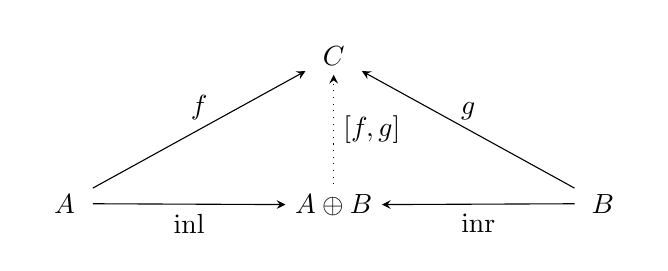
\begin{tikzpicture}
  \matrix (m) [matrix of math nodes,row sep=4em,column sep=7em,minimum width=2em]
  {
   & C &  \\
    A  & A \oplus B & B\\
  };
  \path[-stealth]
    (m-2-1) edge  node [above] {$f$} (m-1-2)
    (m-2-3) edge  node [above] {$g$} (m-1-2)
    (m-2-1) edge  node [below] {$\inl$} (m-2-2)
    (m-2-3) edge  node [below] {$\inr$} (m-2-2)
    (m-2-2) edge [dotted]  node [right] {$[f,g]$} (m-1-2);
    ;
\end{tikzpicture}
\]
\end{definition}

\begin{definition}
        A monoidal category $\catC$ with coproducts is called
        distributive if for every object $A$ in $\catC$ the
        functor $- \otimes A$ preserves coproducts. Explicitly
        this means that the morphism,
        \[
                [\inl \otimes \id, \inr \otimes \id] : B \otimes A \oplus C \otimes                     A \to (B \oplus C) \otimes A
        \]
        is actually as isomorphism. We will denote the respective inverse
        by $\dist$. Note that if $\catC$ is monoidal closed then it is automatically
        distributive as left adjoints preserve all colimits.
\end{definition}

% Let $\mathcal{C}$ be a monoidal closed category and let $X,$ $Y,$ and $Z$ be objects in $\mathcal{C}$. The morphism $\text{dist}_{X, Y,Z}: X \otimes  \left(Y \oplus Z\right) \xrightarrow{} \left(X \otimes Y\right) \oplus \left(X \otimes Y\right)$, denotes the distributive property of the tensor product over the coproduct.  This distributive property holds in monoidal closed categories with coproducts because the tensor functor is a left adjoint (to the internal hom), and left adjoints preserve colimits.

Before presenting the interpretation of $\lambda$-calculus with conditionals in
distributive symmetric monoidal (closed) categories let us give some examples
of the latter in order to illustrate our work's broad range of applicability.

\begin{example}
Examples of monoidal closed categories with coproducts include the category of sets, the category of vector spaces, and the category of partial orders. In the category of sets, the tensor product is the cartesian product, the monoidal unit is the singleton set, the coproduct is the disjoint union, and the internal hom consists of all functions between sets. For the category of vector spaces, the tensor product is the standard tensor product of vector spaces, the monoidal unit is the field of scalars, the coproduct is the direct sum, and the internal hom is the space of linear maps. In the category of partial orders, the tensor product corresponds to the meet ($\wedge$), the monoidal unit to the the singleton poset, the coproduct to the join ($\vee$), and the internal hom is the poset of monotone functions ordered pointwise.
\end{example}

We now present the interpretation of $\lambda$-calculus with conditionals.
First the new type $A \oplus B$ is interpreted as $\sem{A \oplus B} = [\![A
]\!] \oplus [\![ B ]\!]$. As for the new terms, the corresponding
interpretation is defined inductively in \autoref{fig:denotational_sem cond}.

\begin{figure}[H]
  \begin{equation*}
  \begin{aligned}
  &\hspace{10pt}
  %
  \begin{prooftree}
      \hypo{ [\![\Gamma \triangleright v: \mathbb{A}]\!] = m }
      \infer1[]{ [\![ \Gamma \triangleright \text{inl}_{\mathbb{B}} (v):  \mathbb{A} \oplus \mathbb{B}  ]\!] = \inl  \comp m}
  \end{prooftree}
  %
  \hspace{120pt}
  %
  \begin{prooftree}
    \hypo{ [\![\Gamma \triangleright v: \mathbb{B}]\!] = m }
    \infer1[]{ [\![ \Gamma \triangleright \text{inr}_{\mathbb{A}} (v):  \mathbb{A} \oplus \mathbb{B}  ]\!] = \inr  \comp m}
\end{prooftree}
  %
  \\[20pt]
  &\hspace{-20pt}
  %
  \begin{prooftree}
      \hypo{[\![\Gamma\triangleright v: \mathbb{A} \oplus \mathbb{B} ]\!] = b}
      \hypo{[\![\Delta, x:\mathbb{A} \triangleright w: \mathbb{D} ]\!] = p}
      \hypo{ [\![\Delta,y:\mathbb{B} \triangleright u: \mathbb{D} ]\!] = q }
      \hypo{E \in \Shuff(\Gamma; \Delta)}
      \infer4[]{ [\![E \vljud \text{case } v \hspace{2pt}  \{\text{inl}_{\mathbb{B}} (x) \Rightarrow w ; \hspace{1pt} \text{inr}_{\mathbb{A}} (y) \Rightarrow u\}: \mathbb{D} ]\!] =   [p,q] \comp (\text{jn}_{\Delta;\typeA}\comp \sw \oplus \text{jn}_{\Delta;\mathbb{B}}\comp \sw) \comp \dist \comp (b \otimes \text{id}) \cdot \text{sp}_{\Gamma;\Delta} \cdot \text{sh}_{E}}
  \end{prooftree}
  %
  \\[10pt]
  \end{aligned}
  \end{equation*}
  \caption{Judgment interpretation for conditionals}
\label{fig:denotational_sem cond}
\end{figure}

The next step is to demonstrate that the equations in Figure \ref{fig:equations-in-context-cond} are valid under the given interpretation. To achieve this, we first establish the following lemma.

\begin{lemma} \label{lem_interpret_exch:sub} (\text{Exchange and Subsitution}) For all judgements $\Gamma,x:\mathbb{A}, y:\mathbb{B}, \Delta \triangleright v: \mathbb{D}$, $\Gamma,x:\mathbb{A} \triangleright v: \mathbb{B}$ and $\Delta \triangleright w: \mathbb{A}$  the following equations hold: 
  \begin{equation*}
\begin{split}
  [\![\Gamma,x:\mathbb{A}, y:\mathbb{B}, \Delta \triangleright v: \mathbb{D}]\!] = [\![\Gamma,y:\mathbb{B},x:\mathbb{A},  \Delta \triangleright v: \mathbb{D}]\! ] \cdot \text{exch}_{\Gamma, \underline{ \mathbb{A}, \mathbb{B}} ,\Delta} \\
  [\![\Gamma, \Delta \triangleright v[w/x]: \mathbb{B}]\!] = [\![\Gamma, x:\mathbb{A} \triangleright v: \mathbb{B}]\!]\cdot \text{jn}_{\Gamma;\mathbb{A}} \cdot (\text{id} \otimes [\![ \Delta  \triangleright w: \mathbb{A}]\!] ) \cdot \text{sp}_{\Gamma;\Delta} 
\end{split}
  \end{equation*}
\end{lemma}

\begin{proof}
  We begin once again with the exchange property, which follows by induction over the length of derivation trees. The rules involving injections are straightforward. With respect to the rule (case), we distinguish between the scenarios where both variables ($x : \typeA$ and $y : \typeB$) are in $\Gamma$, both are in $\Delta$, or they are distributed across $\Gamma$ and $\Delta$.
  The fist case follows by induction, the bifunctoriality of the tensor product, and the coherence theorem for symmetric monoidal categories.

  %\begin{align*}
    %& [\![\Gamma,x:\mathbb{A}, y:\mathbb{B}, \Delta \triangleright \text{ case }  v \hspace{2pt}  \{\text{inl}_{\mathbb{E}} (a) \Rightarrow w ; \hspace{1pt} \text{inr}_{\mathbb{E}} (b) \Rightarrow u\}: \mathbb{D}]\!] \\ 
    %&\triangleq    \left[ [\![ E, a:\mathbb{D} \triangleright w:\typeD ]\!] \cdot \text{jn}_{E;\mathbb{D}},[\![ E, b:\mathbb{E} \triangleright u:\typeD]\!]\cdot \text{jn}_{E;\mathbb{E} }\right] \cdot \text{dist} \cdot \text{sw}  \\
    %& \hspace{10pt} \cdot ([\![\Gamma_{1},x:\mathbb{A}, y:\mathbb{B},\Gamma_{2} \triangleright v : \mathbb{D} \oplus \mathbb{E}  ]\!] \otimes \text{id})  \cdot \text{sp}_{\Gamma_{1},\mathbb{A}, \mathbb{B},\Gamma_{2};E} \cdot \text{sh}_{\Gamma,\mathbb{A}, \mathbb{B},\Delta} \\
    %& =  \left[ [\![ E, a:\mathbb{D} \triangleright w:\typeD ]\!] \cdot \text{jn}_{E;\mathbb{D}},[\![ E, b:\mathbb{E} \triangleright u:\typeD]\!]\cdot \text{jn}_{E;\mathbb{E} }\right] \cdot \text{dist} \cdot \text{sw}  \\
    %&  \hspace{10pt} \cdot ([\![\Gamma_{1}, y:\mathbb{B},x:\mathbb{A},\Gamma_{2} \triangleright v: \mathbb{D}]\! ]\cdot \hspace{1pt} \text{exch}_{\Gamma_{1}, \underline{\mathbb{A},\mathbb{B}},\Gamma_{2}} \otimes \text{id}) \cdot \text{sp}_{\Gamma_{1},\mathbb{A}, \mathbb{B},\Gamma_{2};E} \cdot \text{sh}_{\Gamma,\mathbb{A}, \mathbb{B},\Delta} \\
    %&  = \left[ [\![ E, a:\mathbb{D} \triangleright w:\typeD ]\!] \cdot \text{jn}_{E;\mathbb{D}},[\![ E, b:\mathbb{E} \triangleright u:\typeD]\!]\cdot \text{jn}_{E;\mathbb{E} }\right]  \cdot \text{dist} \cdot \text{sw}    \\
    %& \hspace{10pt} \cdot ([\![\Gamma_{1}, y:\mathbb{B},x:\mathbb{A},\Gamma_{2} \triangleright v : \mathbb{D} \oplus \mathbb{E}  ]\!]\otimes \text{id}) \cdot (\text{exch}_{\Gamma,  \underline{\mathbb{A},  \mathbb{B}}, \Delta} \otimes \text{id}) \cdot \text{sp}_{\Gamma_{1},\mathbb{A},\mathbb{B}, \Gamma_{2};E}  \cdot \text{sh}_{\Gamma,\mathbb{A}, \mathbb{B},\Delta} & {\text{(bifunctoriality of $\otimes$)}} \\
    %& =   \left[ [\![ E, a:\mathbb{D} \triangleright w:\typeD ]\!] \cdot \text{jn}_{E;\mathbb{D}},[\![ E, b:\mathbb{E} \triangleright u:\typeD]\!]\cdot \text{jn}_{E;\mathbb{E} }\right]  \cdot \text{dist} \cdot \text{sw}  \\
    %& \hspace{10pt} \cdot ([\![\Gamma_{1}, y:\mathbb{B},x:\mathbb{A},\Gamma_{2}  \triangleright v : \mathbb{D} \oplus \mathbb{E}  ]\!]\otimes \text{id}) \cdot \text{sp}_{\Gamma_{1},\mathbb{B},\mathbb{A}, \Gamma_{2};E}  \cdot \text{sh}_{\Gamma,\mathbb{B}, \mathbb{A},\Delta}  \cdot \text{exch}_{\Gamma,  \underline{\mathbb{A},\mathbb{B}}, \Delta} & {\text{(coherence theorem)}} \\
    %& \triangleq   [\![\Gamma,y:\mathbb{B}, x:\mathbb{A}, \Delta \triangleright \text{ case } v \hspace{2pt}  \{\text{inl}_{\mathbb{E}} (a) \Rightarrow w ; \hspace{1pt} \text{inr}_{\mathbb{E}} (b) \Rightarrow u\}: \mathbb{D}]\!] \cdot \text{exch}_{\Gamma,  \underline{\mathbb{A}, \mathbb{B}}, \Delta}
  %\end{align*}


  \begin{align*}
    & [\![\Gamma,x:\mathbb{A}, y:\mathbb{B}, \Delta \triangleright \text{ case }  v \hspace{2pt}  \{\text{inl}_{\mathbb{E}} (a) \Rightarrow w ; \hspace{1pt} \text{inr}_{\mathbb{D}} (b) \Rightarrow u\}: \mathbb{F}]\!] \\ 
    &\triangleq    \left[ [\![  w]\!] \cdot \text{jn}_{E;\mathbb{D}},[\![u]\!]\cdot \text{jn}_{E;\mathbb{E} }\right] \cdot \text{dist} \cdot \text{sw}   \cdot ([\![ v  ]\!] \otimes \text{id})  \cdot \text{sp}_{\Gamma_{1},\mathbb{A}, \mathbb{B},\Gamma_{2};E} \cdot \text{sh}_{\Gamma,\mathbb{A}, \mathbb{B},\Delta} \\
    & =  \left[ [\![  w]\!] \cdot \text{jn}_{E;\mathbb{D}},[\![u]\!]\cdot \text{jn}_{E;\mathbb{E} }\right] \cdot \text{dist} \cdot \text{sw}  \cdot ([\![v]\! ]\cdot \hspace{1pt} \text{exch}_{\Gamma_{1}, \underline{\mathbb{A},\mathbb{B}},\Gamma_{2}} \otimes \text{id}) \cdot \text{sp}_{\Gamma_{1},\mathbb{A}, \mathbb{B},\Gamma_{2};E} \cdot \text{sh}_{\Gamma,\mathbb{A}, \mathbb{B},\Delta} \\
    &  = \left[ [\![w]\!] \cdot \text{jn}_{E;\mathbb{D}},[\![u]\!]\cdot \text{jn}_{E;\mathbb{E} }\right]  \cdot \text{dist} \cdot \text{sw}   \cdot ([\![ v ]\!]\otimes \text{id}) \cdot (\text{exch}_{\Gamma,  \underline{\mathbb{A},  \mathbb{B}}, \Delta} \otimes \text{id}) \cdot \text{sp}_{\Gamma_{1},\mathbb{A},\mathbb{B}, \Gamma_{2};E}  & {\text{(bifunctoriality of $\otimes$)}}\\
    & \hspace{10pt} \cdot  \text{sh}_{\Gamma,\mathbb{A}, \mathbb{B},\Delta} \\
    & =   \left[ [\![ w]\!] \cdot \text{jn}_{E;\mathbb{D}},[\![u]\!]\cdot \text{jn}_{E;\mathbb{E} }\right]  \cdot \text{dist} \cdot \text{sw}  \cdot ([\![v]\!]\otimes \text{id}) \cdot \text{sp}_{\Gamma_{1},\mathbb{B},\mathbb{A}, \Gamma_{2};E}  \cdot \text{sh}_{\Gamma,\mathbb{B}, \mathbb{A},\Delta}  \cdot \text{exch}_{\Gamma,  \underline{\mathbb{A},\mathbb{B}}, \Delta} & {\text{(coherence )}} \\
    & \triangleq   [\![\Gamma,y:\mathbb{B}, x:\mathbb{A}, \Delta \triangleright \text{ case } v \hspace{2pt}  \{\text{inl}_{\mathbb{E}} (a) \Rightarrow w ; \hspace{1pt} \text{inr}_{\mathbb{D}} (b) \Rightarrow u\}: \mathbb{F}]\!] \cdot \text{exch}_{\Gamma,  \underline{\mathbb{A}, \mathbb{B}}, \Delta}
  \end{align*}


The second case follows by induction, the coherence theorem for symmetric monoidal categories, the universal property of the coproduct, and naturality of $\alpha,$ $\lambda,$ $\rho,$ and $\text{sw}$ and their inverses.

\begin{align*}
  & [\![\Gamma,x:\mathbb{A}, y:\mathbb{B}, \Delta \triangleright \text{ case }  \hspace{2pt}  \{\text{inl}_{\mathbb{E}} (a) \Rightarrow w ; \hspace{1pt} \text{inr}_{\mathbb{D}} (b) \Rightarrow u\}: \mathbb{F}]\!] \\
  & \triangleq    \left[[\![ w ]\!] \cdot  \text{jn}_{\Delta_{1},\mathbb{A},\mathbb{B},  \Delta_{2};\mathbb{D}},[\![ u ]\!] \cdot  \text{jn}_{\Delta_{1},\mathbb{A},\mathbb{B},  \Delta_{2};\mathbb{E}}\right]   \cdot \text{dist} \cdot \text{sw} \cdot ([\![v]\!] \otimes \text{id}) \cdot \text{sp}_{E; \Delta_{1},\mathbb{A},\mathbb{B},  \Delta_{2}} \cdot \text{sh}_{\Gamma;\mathbb{A}, \mathbb{B},\Delta}  \\
  & = [[\![ w ]\!]  \cdot \text{exch}_{\Delta_{1},\underline{\mathbb{A},\mathbb{B}},  \Delta_{2},\mathbb{D}} \cdot \text{jn}_{\Delta_{1},\mathbb{A},\mathbb{B},  \Delta_{2};\mathbb{D}},    [\![u ]\!] \cdot \text{exch}_{\Delta_{1},\underline{\mathbb{A},\mathbb{B}},  \Delta_{2},\mathbb{E}} \cdot \text{jn}_{\Delta_{1},\mathbb{A},\mathbb{B},  \Delta_{2};\mathbb{E}} ] \cdot \text{dist} \cdot \text{sw} \\
  & \hspace{10pt} \cdot ([\![  v : \mathbb{D} \oplus \mathbb{E}  ]\!] \otimes \text{id}) \cdot\text{sp}_{E; \Delta_{1},\mathbb{A},\mathbb{B},  \Delta_{2}} \cdot \text{sh}_{\Gamma,\mathbb{A}, \mathbb{B},\Delta} \\
  & = [[\![ w ]\!] \cdot \text{jn}_{\Delta_{1} ,\mathbb{B},\mathbb{A},  \Delta_{2};\mathbb{D}} \cdot \text{sp}_{\Delta_{1}, \mathbb{B}, \mathbb{A}, \Delta_{2};\mathbb{D}} \cdot  \text{exch}_{\Delta_{1},\underline{\mathbb{A},\mathbb{B}},  \Delta_{2},\mathbb{D}} \cdot  \text{jn}_{\Delta_{1},\mathbb{A},\mathbb{B},  \Delta_{2};\mathbb{D}}  ,    [\![u ]\!] \cdot \text{jn}_{\Delta_{1} ,\mathbb{B},\mathbb{A},  \Delta_{2};\mathbb{E}} & {\text{(coherence )}} \\
  & \hspace{10pt} \cdot \text{sp}_{\Delta_{1}, \mathbb{B}, \mathbb{A}, \Delta_{2};\mathbb{E}} \cdot  \text{exch}_{\Delta_{1},\underline{\mathbb{A},\mathbb{B}},  \Delta_{2},\mathbb{E}} \cdot  \text{jn}_{\Delta_{1},\mathbb{A},\mathbb{B},  \Delta_{2};\mathbb{E}} ] \cdot \text{dist} \cdot \text{sw} \cdot ([\![  v : \mathbb{D} \oplus \mathbb{E}  ]\!] \otimes \text{id}) \\
  & \hspace{10pt} \cdot\text{sp}_{E; \Delta_{1},\mathbb{A},\mathbb{B},  \Delta_{2}} \cdot \text{sh}_{\Gamma,\mathbb{A}, \mathbb{B},\Delta} \\
  & = [[\![ w ]\!] \cdot \text{jn}_{\Delta_{1} ,\mathbb{B},\mathbb{A},  \Delta_{2};\mathbb{D}},  [\![u ]\!] \cdot \text{jn}_{\Delta_{1} ,\mathbb{B},\mathbb{A},  \Delta_{2};\mathbb{E}}] \cdot [ i_1 \cdot  \text{sp}_{\Delta_{1}, \mathbb{B}, \mathbb{A}, \Delta_{2};\mathbb{D}} \cdot  \text{exch}_{\Delta_{1},\underline{\mathbb{A},\mathbb{B}},  \Delta_{2},\mathbb{D}} \cdot  & {\text{(law of coproducts)}} \\
  & \hspace{10pt}  \text{jn}_{\Delta_{1},\mathbb{A},\mathbb{B},  \Delta_{2},\mathbb{D}},  i_2 \cdot  \text{sp}_{\Delta_{1}, \mathbb{B}, \mathbb{A}, \Delta_{2};\mathbb{E}} \cdot  \text{exch}_{\Delta_{1},\underline{\mathbb{A},\mathbb{B}},  \Delta_{2};\mathbb{E}} \cdot  \text{jn}_{\Delta_{1},\mathbb{A},\mathbb{B},  \Delta_{2};\mathbb{E}} ] \cdot \text{dist} \cdot \text{sw} \cdot ([\![  v : \mathbb{D} \oplus \mathbb{E}  ]\!] \\
  & \hspace{10pt} \otimes \text{id})  \cdot\text{sp}_{E; \Delta_{1},\mathbb{A},\mathbb{B},  \Delta_{2}} \cdot \text{sh}_{\Gamma,\mathbb{A}, \mathbb{B},\Delta} \\ 
\end{align*}
The commutativity of the following diagram follows from the universal property of the coproduct and the naturality of $\alpha,$ $\lambda,$ $\rho,$ and $\text{sw}$, their inverses, and their composition. Here $\phi$ corresponds to $\text{sp}_{\Delta_{1}, \mathbb{B}, \mathbb{A}, \Delta_{2}; \mathbb{D} \oplus\mathbb{E}} \cdot  \text{exch}_{\Delta_{1},\underline{\mathbb{A},\mathbb{B}},  \Delta_{2}, \mathbb{D} \oplus\mathbb{E}} \cdot  \text{jn}_{\Delta_{1},\mathbb{A},\mathbb{B},  \Delta_{2}; \mathbb{D} \oplus\mathbb{E}}$, $\phi_1$ to $\text{sp}_{\Delta_{1}, \mathbb{B}, \mathbb{A}, \Delta_{2}; \mathbb{D}} \cdot  \text{exch}_{\Delta_{1},\underline{\mathbb{A},\mathbb{B}},  \Delta_{2}, \mathbb{D}} \cdot  \text{jn}_{\Delta_{1},\mathbb{A},\mathbb{B},  \Delta_{2}; \mathbb{D}}$, and $\phi_2$ to $\text{sp}_{\Delta_{1}, \mathbb{B}, \mathbb{A}, \Delta_{2}; \mathbb{E}} \cdot  \text{exch}_{\Delta_{1},\underline{\mathbb{A},\mathbb{B}},  \Delta_{2}, \mathbb{E}} \cdot  \text{jn}_{\Delta_{1},\mathbb{A},\mathbb{B},  \Delta_{2}; \mathbb{E}}$.


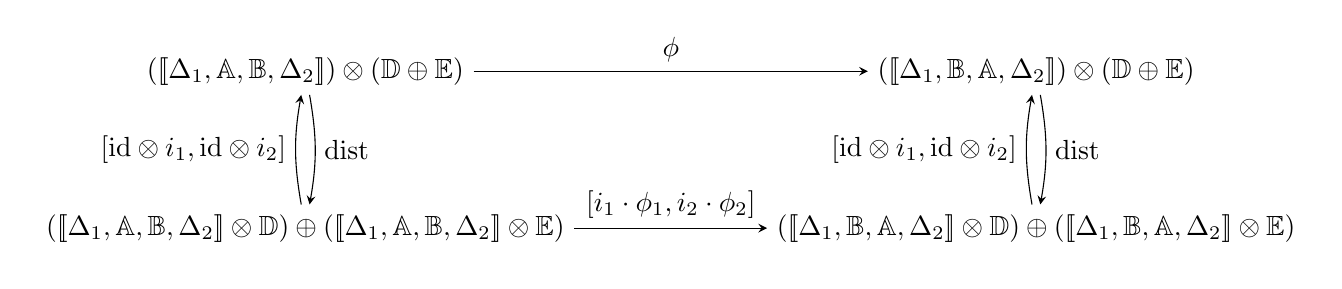
\begin{tikzpicture}
  \matrix (m) [matrix of math nodes,row sep=4em,column sep=7em,minimum width=2em]
  {
    \left([\![ \Delta_{1},\mathbb{A},\mathbb{B}, \Delta_{2} ]\!]\right)  \otimes  (\mathbb{D} \oplus \mathbb{E})  &   \left([\![ \Delta_{1},\mathbb{B},\mathbb{A}, \Delta_{2} ]\!]\right)  \otimes  (\mathbb{D} \oplus \mathbb{E})   \\
    \left([\![ \Delta_{1},\mathbb{A},\mathbb{B}, \Delta_{2} ]\!]  \otimes \mathbb{D}\right) \oplus \left([\![ \Delta_{1},\mathbb{A},\mathbb{B}, \Delta_{2} ]\!]  \otimes \mathbb{E}\right)  &  \left([\![ \Delta_{1},\mathbb{B},\mathbb{A}, \Delta_{2} ]\!]  \otimes \mathbb{D}\right) \oplus \left([\![ \Delta_{1},\mathbb{B},\mathbb{A}, \Delta_{2} ]\!]  \otimes \mathbb{E}\right) \\
  };
  \path[-stealth]
    (m-1-1) edge node [above] {$ \phi$} (m-1-2)
    (m-2-1)  edge[bend right=-10] node [pos=0.5, shift={(-1.3, 0)}] {$[\text{id} \otimes i_1,\text{id} \otimes i_2]$} (m-1-1)
    (m-1-1) edge [bend left=10] node [pos=0.5, shift={(0.4,0)}] {$\text{dist}$} (m-2-1)
    (m-2-1) edge node [above] {$ [i_1 \cdot \phi_1, i_2 \cdot \phi_2 ]$} (m-2-2)
    (m-1-2) edge [bend left=10] node [pos=0.5, shift={(0.4,0)}] {$\text{dist}$} (m-2-2)
    (m-2-2)  edge[bend right=-10] node [pos=0.5, shift={(-1.3, 0)}] {$[\text{id} \otimes i_1,\text{id} \otimes i_2]$} (m-1-2)
    ;
\end{tikzpicture}
 
As a result it holds that 
\begin{align*}
  & [[\![ w ]\!] \cdot \text{jn}_{\Delta_{1} ,\mathbb{B},\mathbb{A},  \Delta_{2};\mathbb{D}},  [\![u ]\!] \cdot \text{jn}_{\Delta_{1} ,\mathbb{B},\mathbb{A},  \Delta_{2};\mathbb{E}}] \cdot [ i_1 \cdot  \text{sp}_{\Delta_{1}, \mathbb{B}, \mathbb{A}, \Delta_{2};\mathbb{D}} \cdot  \text{exch}_{\Delta_{1},\underline{\mathbb{A},\mathbb{B}},  \Delta_{2},\mathbb{D}} \cdot   \\
  & \hspace{10pt}  \text{jn}_{\Delta_{1},\mathbb{A},\mathbb{B},  \Delta_{2},\mathbb{D}},  i_2 \cdot  \text{sp}_{\Delta_{1}, \mathbb{B}, \mathbb{A}, \Delta_{2};\mathbb{E}} \cdot  \text{exch}_{\Delta_{1},\underline{\mathbb{A},\mathbb{B}},  \Delta_{2};\mathbb{E}} \cdot  \text{jn}_{\Delta_{1},\mathbb{A},\mathbb{B},  \Delta_{2};\mathbb{E}} ] \cdot \text{dist} \cdot \text{sw} \cdot ([\![  v : \mathbb{D} \oplus \mathbb{E}  ]\!] \\
  & \hspace{10pt} \otimes \text{id})  \cdot\text{sp}_{E; \Delta_{1},\mathbb{A},\mathbb{B},  \Delta_{2}} \cdot \text{sh}_{\Gamma,\mathbb{A}, \mathbb{B},\Delta} \\ 
  & = [[\![ w ]\!] \cdot \text{jn}_{\Delta_{1} ,\mathbb{B},\mathbb{A},  \Delta_{2};\mathbb{D}},  [\![u ]\!] \cdot \text{jn}_{\Delta_{1} ,\mathbb{B},\mathbb{A},  \Delta_{2};\mathbb{E}}] \cdot \text{dist} \cdot \text{sp}_{\Delta_{1}, \mathbb{B}, \mathbb{A}, \Delta_{2}; \mathbb{D} \oplus\mathbb{E}} \cdot  \text{exch}_{\Delta_{1},\underline{\mathbb{A},\mathbb{B}},  \Delta_{2}, \mathbb{D} \oplus\mathbb{E}}\\
  & \hspace{10pt}  \cdot  \text{jn}_{\Delta_{1},\mathbb{A},\mathbb{B},  \Delta_{2}; \mathbb{D} \oplus\mathbb{E}}  \cdot \text{sw} \cdot ([\![  v : \mathbb{D} \oplus \mathbb{E}  ]\!] \otimes \text{id})  \cdot\text{sp}_{E; \Delta_{1},\mathbb{A},\mathbb{B},  \Delta_{2}} \cdot \text{sh}_{\Gamma,\mathbb{A}, \mathbb{B},\Delta}\\
  & = [[\![ w ]\!] \cdot \text{jn}_{\Delta_{1} ,\mathbb{B},\mathbb{A},  \Delta_{2};\mathbb{D}},  [\![u ]\!] \cdot \text{jn}_{\Delta_{1} ,\mathbb{B},\mathbb{A},  \Delta_{2};\mathbb{E}}] \cdot \text{dist} \cdot \text{sw} \cdot \text{sp}_{\mathbb{D} \oplus\mathbb{E};\Delta_{1}, \mathbb{B}, \mathbb{A}, \Delta_{2}} \cdot  \text{exch}_{\mathbb{D} \oplus\mathbb{E}, \Delta_{1},\underline{\mathbb{A},\mathbb{B}},  \Delta_{2}} & {\text{(naturality of sw)}} \\
  & \hspace{10pt} \cdot  \text{jn}_{\mathbb{D} \oplus\mathbb{E};\Delta_{1},\mathbb{A},\mathbb{B},  \Delta_{2}} \cdot ([\![  v : \mathbb{D} \oplus \mathbb{E}  ]\!] \otimes \text{id})  \cdot\text{sp}_{E; \Delta_{1},\mathbb{A},\mathbb{B},  \Delta_{2}} \cdot \text{sh}_{\Gamma,\mathbb{A}, \mathbb{B},\Delta} \\
  & = [[\![ w ]\!] \cdot \text{jn}_{\Delta_{1} ,\mathbb{B},\mathbb{A},  \Delta_{2};\mathbb{D}},  [\![u ]\!] \cdot \text{jn}_{\Delta_{1} ,\mathbb{B},\mathbb{A},  \Delta_{2};\mathbb{E}}] \cdot \text{dist} \cdot \text{sw} \cdot ([\![  v : \mathbb{D} \oplus \mathbb{E}  ]\!] \otimes \text{id}) \cdot \text{sp}_{E;\Delta_{1}, \mathbb{B}, \mathbb{A}, \Delta_{2}} & {\text{(naturality)}} \\
  & \hspace{10pt}  \cdot  \text{exch}_{E, \Delta_{1},\underline{\mathbb{A},\mathbb{B}},  \Delta_{2}} \cdot  \text{jn}_{E ;\Delta_{1},\mathbb{A},\mathbb{B},  \Delta_{2}}   \cdot\text{sp}_{E; \Delta_{1},\mathbb{A},\mathbb{B},  \Delta_{2}} \cdot \text{sh}_{\Gamma,\mathbb{A}, \mathbb{B},\Delta} \\
  & = [[\![ w ]\!] \cdot \text{jn}_{\Delta_{1} ,\mathbb{B},\mathbb{A},  \Delta_{2};\mathbb{D}},  [\![u ]\!] \cdot \text{jn}_{\Delta_{1} ,\mathbb{B},\mathbb{A},  \Delta_{2};\mathbb{E}}] \cdot \text{dist} \cdot \text{sw} \cdot ([\![  v : \mathbb{D} \oplus \mathbb{E}  ]\!] \otimes \text{id}) \cdot \text{sp}_{E; \Delta_{1}, \mathbb{B},\mathbb{A},  \Delta_{2}} & {\text{(coherence)}} \\
  & \hspace{10pt} \cdot \cdot \text{sh}_{\Gamma; \mathbb{B},\mathbb{A}, \Delta} \cdot  \text{exch}_{E, \Delta_{1},\underline{\mathbb{A},\mathbb{B}},  \Delta_{2}} \\
  & \triangleq [\![\Gamma,y:\mathbb{B}, x:\mathbb{A}, \Delta \triangleright \text{ case }  \hspace{2pt}  \{\text{inl}_{\mathbb{D}} (a) \Rightarrow w ; \hspace{1pt} \text{inr}_{\mathbb{E}} (b) \Rightarrow u\}: \mathbb{F}]\!] \cdot \text{exch}_{\Gamma,\underline{\mathbb{A},  \mathbb{B}}, \Delta}
\end{align*}

For the third case, the proof now follows directly from the implication established in the analogous case of the proof of Lemma \ref{lem:exh_and_sub}, together with the coherence theorem for symmetric monoidal categories.

Regarding the substitution rule, once again the cases involving the injections follow directly by induction on the derivation tree. For the rule (case), we distinguish between the scenarios where the variable $x$ is in $\Gamma$ or in $\Delta$. The first case follows from induction, the bifunctoriality of the tensor product, and the naturality of $\alpha$, $\lambda$, $\rho$, $\text{sw}$, their inverses, and their respective compositions.

\begin{align*}
  &[\![E, Z \triangleright \text{ case } v  \hspace{2pt}  \{\text{inl}_{\mathbb{D}} (a) \Rightarrow w ; \hspace{1pt} \text{inr}_{\mathbb{E}} (b) \Rightarrow u\} [t/x]: \mathbb{B}]\!] \\
  & \triangleq  \left[[\![ w]\!] \cdot \text{jn}_{ \Delta;\mathbb{D}},[\![ u ]\!] \cdot \text{jn}_{ \Delta;\mathbb{E}}\right] \cdot \text{dist} \cdot \text{sw} \cdot ([\![ v [t/x] ]\!]   \otimes \text{id})  \cdot \text{sp}_{\Gamma, Z;\Delta} \cdot \text{sh}_{E,Z} \\
  & = \left[[\![w]\!] \cdot \text{jn}_{ \Delta;\mathbb{D}},[\![u ]\!] \cdot \text{jn}_{ \Delta;\mathbb{E}}\right] \cdot \text{dist} \cdot \text{sw} \cdot (([\![ v]\!]  \cdot \text{jn}_{\Gamma; \mathbb{A}} \cdot (\text{id} \otimes [\![  t ]\!] ) \cdot \text{sp}_{\Gamma;Z} )\otimes \text{id}) \cdot \text{sp}_{\Gamma, Z;\Delta} \\
  & \hspace{10pt} \cdot \text{sh}_{E,Z} \\
  & =  \left[[\![w]\!] \cdot \text{jn}_{ \Delta;\mathbb{D}},[\![u ]\!] \cdot \text{jn}_{ \Delta;\mathbb{E}}\right] \cdot \text{dist} \cdot \text{sw} \cdot ([\![ v]\!] \otimes \text{id}) \cdot (\text{jn}_{\Gamma; \mathbb{A}} \cdot (\text{id} \otimes [\![  t ]\!] ) \cdot \text{sp}_{\Gamma;Z} \otimes \text{id}) \cdot \text{sp}_{\Gamma, Z;\Delta}  & {\text{(bifunctoriality of $\otimes$)}} \\
  & \hspace{10pt} \cdot \text{sh}_{E,Z}\\
  & = \left[[\![w]\!] \cdot \text{jn}_{ \Delta;\mathbb{D}},[\![u ]\!] \cdot \text{jn}_{ \Delta;\mathbb{E}}\right] \cdot \text{dist} \cdot \text{sw} \cdot ([\![ v]\!] \otimes \text{id}) \cdot \text{sp}_{\Gamma, \typeA;\Delta}  \cdot \text{sh}_{E,\typeA}  \cdot  \text{jn}_{E; \typeA} \cdot (\text{id} \otimes [\![ t ]\!] ) \cdot \text{sp}_{E;Z}  & {(\text{naturality})}   \\
  & \triangleq  \hspace{2pt} [\![E,  x:\mathbb{A} \triangleright \text{ case } v \hspace{2pt}  \{\text{inl}_{\mathbb{B}} (x) \Rightarrow w ; \hspace{1pt} \text{inr}_{\mathbb{D}} (y) \Rightarrow u\}: \mathbb{E}]\!]  \cdot  \text{jn}_{E; \typeA} \cdot (\text{id} \otimes [\![ t ]\!] ) \cdot \text{sp}_{E;Z}
\end{align*}


The second case follows from induction, the exchange rule, the universal property of the coproduct,  the bifunctoriality of the tensor product, and the naturality of $\alpha$, $\lambda$, $\rho$, and $\text{sw}$, along with their inverses and respective compositions.

\begin{align*}
  &[\![E, Z \triangleright \text{ case } v  \hspace{2pt}  \{\text{inl}_{\mathbb{D}} (a) \Rightarrow w ; \hspace{1pt} \text{inr}_{\mathbb{E}} (b) \Rightarrow u\} [t/x]: \mathbb{B}]\!] \\
  & \triangleq  \left[[\![ \Delta  , Z ,  a:\mathbb{D} \triangleright w[t/x] ]\!] \cdot \text{jn}_{ \Delta;\mathbb{D}},[\![ \Delta, Z, b:\mathbb{E} \triangleright u[t/x]  ]\!] \cdot \text{jn}_{ \Delta;\mathbb{E}}\right] \cdot \text{dist} \cdot \text{sw} \cdot ([\![ v ]\!]   \otimes \text{id})  \\
  &  \hspace{10pt}  \cdot \text{sp}_{\Gamma, Z;\Delta} \cdot \text{sh}_{E,Z} \hspace{10pt} \\
  & =   [[\![ \Delta ,  a:\mathbb{D} , Z \triangleright  w [t/x]  ]\!] \cdot \text{exch}_{\Delta,Z,\mathbb{D}} \cdot \text{jn}_{\Delta, Z; \mathbb{D}},[\![  \Delta ,  b:\mathbb{E} , Z \triangleright u [a/z]   ]\!] \cdot \text{exch}_{\Delta, Z,\mathbb{E}}   & {(\text{exchange})} \\
  & \hspace{10pt} \cdot \text{jn}_{\Delta, Z; \mathbb{E}} ] \cdot \text{dist} \cdot \text{sw} \cdot ([\![v]\!] \otimes \text{id})  \cdot \text{sp}_{\Gamma; \Delta, Z} \cdot \text{sh}_{E,Z}    \\
  & =  [[\![ w ]\!]  \cdot \text{jn}_{\Delta,\mathbb{D}; \mathbb{A}} \cdot (\text{id} \otimes [\![t]\!] ) \cdot \text{sp}_{\Delta,\mathbb{D}; \mathbb{A}} \cdot  \text{exch}_{\Delta, Z,\mathbb{D}} \cdot \text{jn}_{\Delta, Z; \mathbb{D}} , [\![ u ]\!]\cdot \text{jn}_{\Delta,\mathbb{E}; \mathbb{A}} \cdot (\text{id} \otimes [\![ t]\!] )     \\
  & \hspace{10pt} \cdot \text{sp}_{\Delta,\mathbb{E}; \mathbb{A}}  \cdot \text{exch}_{\Delta, Z,\mathbb{E}} \cdot\text{jn}_{\Delta Z, \mathbb{E}} ]\cdot \text{dist} \cdot \text{sw} \cdot ([\![v]\!] \otimes \text{id})  \cdot \text{sp}_{\Gamma; \Delta, Z} \cdot \text{sh}_{E,Z} \\
  & = [[\![ w ]\!] \cdot \text{exch}_{\Delta, \mathbb{A},\mathbb{D}} \cdot \text{jn}_{\Delta, \mathbb{A}; \mathbb{D}} \cdot (\text{jn}_{\Delta; \mathbb{A}} \otimes \text{id}) \cdot (\text{id} \otimes [\![t]\!]  \otimes \text{id}) \cdot  (\text{sp}_{\Delta; Z} \otimes \text{id}),  [\![ u ]\!]  & {(\text{naturality})} \\
  & \hspace{10pt} \cdot \text{exch}_{\Delta, \mathbb{A},\mathbb{E}} \cdot \text{jn}_{\Delta, \mathbb{A}; \mathbb{E}} \cdot (\text{jn}_{\Delta; \mathbb{A}} \otimes \text{id}) \cdot (\text{id} \otimes [\![t]\!]  \otimes \text{id}) \cdot  (\text{sp}_{\Delta; Z} \otimes \text{id}) ] \cdot \text{dist} \cdot \text{sw}  \\
  &  \hspace{10pt} \cdot ([\![v]\!] \otimes \text{id})  \cdot \text{sp}_{\Gamma; \Delta, Z} \cdot \text{sh}_{E,Z} \\
  & = [[\![ \Delta  , x:\mathbb{A} ,  a:\mathbb{D} \triangleright w]\!] \cdot \text{jn}_{\Delta, \mathbb{A}; \mathbb{D}}, [\![ \Delta  , x:\mathbb{A} ,  b:\mathbb{E} \triangleright u]\!] \cdot \text{jn}_{\Delta, \mathbb{A}; \mathbb{E}}]  \cdot [i_1  \cdot  (\text{jn}_{\Delta; \mathbb{A}} \otimes \text{id})     & {(\text{exchange and }}  \\
  & \hspace{10pt} \cdot (\text{id} \otimes [\![t]\!]  \otimes \text{id})  \cdot (\text{sp}_{\Delta; Z} \otimes \text{id}), i_2 \cdot (\text{jn}_{\Delta; \mathbb{A}} \otimes \text{id})   \cdot (\text{id} \otimes [\![t]\!]  \otimes \text{id}) \cdot  (\text{sp}_{\Delta; Z} \otimes \text{id})] \cdot \text{dist}  & { \text{coprodut})}\\
  & \hspace{10pt} \cdot \text{sw} \cdot ([\![v]\!] \otimes \text{id})  \cdot \text{sp}_{\Gamma; \Delta, Z} \cdot \text{sh}_{E,Z} \\
  &= [[\![w]\!] \cdot \text{jn}_{\Delta, \mathbb{A}; \mathbb{D}}, [\![u]\!] \cdot \text{jn}_{\Delta, \mathbb{A}; \mathbb{E}}]  \cdot \text{dist} \cdot (\text{jn}_{\Delta; \mathbb{A}} \otimes \text{id})   \cdot (\text{id} \otimes [\![t]\!]  \otimes \text{id}) \cdot  (\text{sp}_{\Delta; Z} \otimes \text{id}) \cdot \text{sw}  & {(\text{coproduct, naturality, }}  \\
  & \hspace{10pt} \cdot ([\![v]\!] \otimes \text{id}) \cdot \text{sp}_{\Gamma; \Delta, Z} \cdot \text{sh}_{E,Z}  & {\text{and bifunctoriality of } \otimes})  \\
  & =  [[\![w]\!] \cdot \text{jn}_{\Delta, \mathbb{A}; \mathbb{D}}, [\![u]\!] \cdot \text{jn}_{\Delta, \mathbb{A}; \mathbb{E}}]  \cdot \text{dist} \cdot \text{sw}  \cdot ([\![v  ]\!] \otimes \text{id}) \cdot \text{sp}_{\Gamma; \Delta, \mathbb{A}} \cdot \text{sh}_{E,\mathbb{A}} \cdot \text{jn}_{E; \mathbb{A}} \cdot (\text{id} \otimes [\![ t  ]\!] ) & {(\text{naturality and  }} \\
  & \hspace{10pt} \cdot \text{sp}_{E;Z} &{\text{and bifunctoriality of } \otimes})  \\ 
  & \triangleq  [\![E,  x:\mathbb{A} \triangleright \text{ case } v \hspace{2pt}  \{\text{inl}_{\mathbb{D}} (a) \Rightarrow w ; \hspace{1pt} \text{inr}_{\mathbb{E}} (b) \Rightarrow u\}: \mathbb{B}]\!] \cdot \text{jn}_{E; \mathbb{A}} \cdot (\text{id} \otimes [\![ t ]\!] ) \cdot \text{sp}_{E;Z}
\end{align*}
\end{proof}

\begin{theorem} \label {theorem:eq_in_context}
  The equations presented in Figure \ref{fig:equations-in-context-cond} are sound w.r.t. judgement interpretation. More specifically if $ \Gamma \triangleright v = w: \typeA$ is one of the equations in Fig. 3 then $[\![ \Gamma \triangleright v: \typeA ]\!] = [\![ \Gamma \triangleright w: \typeA ]\!]$.
\end{theorem}

\begin{proof}
  Follows from Lemma \autoref{lem_interpret_exch:sub}, the coherence theorem for symmetric monoidal categories, naturality,  the bifunctoriality of the tensor product, and the universal property of the coproduct.   
  We will provide a complete proof for the first and third equations, noting that the proof for the second equation follows analogously from the first.
  \begin{align*}
    &\llbracket \Delta,\Gamma \triangleright  \text{ case } v \hspace{2pt} \text{inl}_{\mathbb{B}}(v) \hspace{2pt} \{\text{inl}_{\mathbb{B}} (x) \Rightarrow w ; \hspace{1pt} \text{inr}_{\mathbb{A}} (y) \Rightarrow u\}: \mathbb{D}\rrbracket \\
    & \triangleq  [\llbracket w\rrbracket \cdot \text{jn}_{\Delta;\mathbb{A}},\llbracket u \rrbracket\cdot \text{jn}_{\Delta;\mathbb{B}}] \cdot \text{dist} \cdot \text{sw} \cdot ( i_1 \cdot \llbracket  v \rrbracket \otimes \text{id}) \cdot \text{sp}_{\Gamma;\Delta} \cdot \text{sh}_{\Delta;\Gamma} \\
    & = [\llbracket w\rrbracket \cdot \text{jn}_{\Delta;\mathbb{A}},\llbracket u \rrbracket\cdot \text{jn}_{\Delta;\mathbb{B}}] \cdot \text{dist} \cdot (i_1 \otimes \text{id}) \cdot \text{sw} \cdot ( \llbracket  v \rrbracket \otimes \text{id}) \cdot \text{sp}_{\Gamma;\Delta} \cdot \text{sh}_{\Delta;\Gamma} &{(\text{naturality and bifunctoriality  of } \otimes}) 
  \end{align*}
\end{proof}

Considering the universal property of coproducts, it follows that the following diagram commutes.

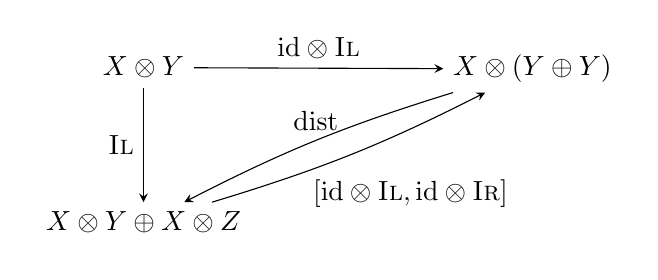
\begin{tikzpicture}
  \matrix (m) [matrix of math nodes,row sep=4em,column sep=7em,minimum width=2em]
  {
    X \otimes Y  &  X \otimes (Y  \oplus Y) \\
     X  \otimes Y \oplus X \otimes Z \\
  };
  \path[-stealth]
    (m-1-1) edge node [left] {$\textsc{Il}$} (m-2-1)
    (m-1-1) edge node [above] {$\text{id} \otimes \textsc{Il}$} (m-1-2)
    (m-2-1) edge[bend right=5] node [pos=0.5, shift={(0.75, -0.5)}] {$[\text{id} \otimes \textsc{Il},\text{id} \otimes \textsc{Ir}]$} (m-1-2)
    (m-1-2) edge[bend left=-5] node [above==0.2cm] {$\text{dist}$} (m-2-1)
    ;
\end{tikzpicture}

As a result, it holds that

\begin{align*}
  & [\llbracket w\rrbracket \cdot \text{jn}_{\Delta;\mathbb{A}},\llbracket u \rrbracket\cdot \text{jn}_{\Delta;\mathbb{B}}] \cdot \text{dist} \cdot (i_1 \otimes \text{id}) \cdot \text{sw} \cdot ( \llbracket  v \rrbracket \otimes \text{id}) \cdot \text{sp}_{\Gamma;\Delta} \cdot \text{sh}_{\Delta;\Gamma} \\
  & = \llbracket  w \rrbracket\cdot \text{jn}_{\Delta;\mathbb{A}} \cdot   \text{sw} \cdot(\llbracket v \rrbracket \otimes  \text{id}) \cdot \text{sp}_{\Gamma;\Delta} \cdot \text{sh}_{\Delta; \Gamma}  & {\text{(law of coproducts)}} \\
  &=  \llbracket  w \rrbracket\cdot \text{jn}_{\Delta;\mathbb{A}}  \cdot(  \text{id}\otimes \llbracket v \rrbracket ) \cdot   \text{sw} \cdot \text{sp}_{\Gamma;\Delta} \cdot \text{sh}_{\Delta; \Gamma} & {\text{(naturality)}} \\
  &= \llbracket w \rrbracket \cdot \text{jn}_{\Delta;\mathbb{A}} \cdot( \text{id} \otimes \llbracket v \rrbracket) \cdot \text{sp}_{\Delta;\Gamma}& {\text{(coherence)}}\\
  & = \llbracket w[v/x] : \mathbb{D} \rrbracket  & {\text{(lemma \ref{lem_interpret_exch:sub})}}
\end{align*}

%\todo[inline,size=\normalsize]{Elitzur‑Vaidman Bomb Testing Problem -> Improve usando o efeito Zeno? -> Acho que não tem ifs} 

Regarding the third equation, we have that
\begin{align*}
  & \llbracket \Delta,\Gamma \triangleright \text{ case } v \hspace{2pt} \{\text{inl}_{\mathbb{B}} (y) \Rightarrow w [ \text{inl}_{\mathbb{B}}(y)/x] ; \hspace{1pt} \text{inr}_{\mathbb{A}} (z) \Rightarrow w [ \text{inr}_{\mathbb{A}}(z)/x]\}: \mathbb{D}\rrbracket \\
  & \triangleq  [\llbracket  w [ \text{inl}_{\mathbb{B}}(y)/x] \rrbracket \cdot \text{jn}_{\Delta;\mathbb{A}} ,\llbracket  w [ \text{inr}_{\mathbb{A}}(z)/x] \rrbracket \cdot \text{jn}_{\Delta;\mathbb{B}} ] \cdot \text{dist} \cdot \text{sw}  \cdot (\llbracket v\rrbracket \otimes \text{id}) \cdot  \text{sp}_{\Gamma;\Delta} \cdot \text{sh}_{\Delta;\Gamma} \\
  & =  [\llbracket w \rrbracket \cdot \text{jn}_{\Delta;\mathbb{A} \oplus \mathbb{B}} \cdot (\text{id} \otimes i_1 \cdot  \llbracket y:\typeA \triangleright y:\typeA  \rrbracket) \cdot \text{sp}_{\Delta;\mathbb{A}} \cdot \text{jn}_{\Delta;\mathbb{A}}, 
  \llbracket w \rrbracket \cdot \text{jn}_{\Delta;\mathbb{A} \oplus \mathbb{B}} \cdot (\text{id} \otimes i_2  & {\text{(lemma \ref{lem_interpret_exch:sub})}} \\
  &  \hspace{10pt} \cdot \llbracket z:\typeB \triangleright z:\typeB  \rrbracket) \cdot \text{sp}_{\Delta;\mathbb{B}} \cdot \text{jn}_{\Delta;\mathbb{B}} ] \cdot \text{dist} \cdot \text{sw} \cdot (\llbracket v\rrbracket \otimes \text{id}) \cdot  \text{sp}_{\Gamma;\Delta} \cdot \text{sh}_{\Delta;\Gamma}  \\
  & = [\llbracket w \rrbracket \cdot \text{jn}_{\Delta;\mathbb{A} \oplus \mathbb{B}} \cdot (\text{id} \otimes i_1) , \llbracket  w \rrbracket  \cdot \text{jn}_{\Delta;\mathbb{A} \oplus \mathbb{B}}   \cdot (\text{id} \otimes i_2) ] \cdot \text{dist} \cdot \text{sw}  \cdot (\llbracket v \oplus \mathbb{B}\rrbracket \otimes \text{id})  \cdot  \text{sp}_{\Gamma;\Delta}  & {\text{(coherence)}}   \\
  & \hspace{10pt}  \cdot \text{sh}_{\Delta;\Gamma} \\
  & = \llbracket w \rrbracket \cdot \text{jn}_{\Delta;\mathbb{A} \oplus \mathbb{B}} \cdot [\text{id} \otimes i_1, \text{id} \otimes i_2] \cdot \text{dist} \cdot \text{sw}  \cdot (\llbracket v \oplus \mathbb{B}\rrbracket \otimes \text{id})  \cdot  \text{sp}_{\Gamma;\Delta} \cdot \text{sh}_{\Delta;\Gamma}  & {\text{(law of coproducts)}}  \\
  & = \llbracket w \rrbracket \cdot \text{jn}_{\Delta;\mathbb{A} \oplus \mathbb{B}} \cdot  \text{id} \cdot \text{sw}  \cdot (\llbracket v \oplus \mathbb{B}\rrbracket \otimes \text{id})  \cdot  \text{sp}_{\Gamma;\Delta} \cdot \text{sh}_{\Delta;\Gamma}  & {\text{(law of coproducts)}}\\
  & = \llbracket w \rrbracket \cdot \text{jn}_{\Delta;\mathbb{A} \oplus \mathbb{B}} \cdot ( \text{id} \otimes \llbracket v \oplus \mathbb{B}\rrbracket )  \cdot  \text{sw}  \cdot  \text{sp}_{\Gamma;\Delta} \cdot \text{sh}_{\Delta;\Gamma}  & {\text{(naturality)}}\\
  &  = \llbracket w \rrbracket \cdot \text{jn}_{\Delta;\mathbb{A} \oplus \mathbb{B}} \cdot ( \text{id} \otimes \llbracket v \oplus \mathbb{B}\rrbracket )  \cdot  \text{sp}_{\Delta; \Gamma} & {\text{(coherence)}}\\
  & \triangleq \llbracket w[v/x] : \mathbb{D} \rrbracket & {\text{(lemma \ref{lem_interpret_exch:sub})}}
\end{align*}

\newpage
\bibliographystyle{alpha} 
\bibliography{biblio}
\end{document}
